\subsection{Introduction}
Differential equations can be split into two big groups:
\begin{itemize}
	\item Ordinary differential equations (ODE)
	\begin{itemize}
		\setlength\itemsep{0.5em}
		\item Single ODE
		\item System of ODEs
	\end{itemize}
	\item Partial differential equations (PDE)
	\begin{itemize}
		\setlength\itemsep{0.5em}
		\item Single PDE
		\item System of PDEs
	\end{itemize}
\end{itemize}
For each group or class of equations, there are many solution methods: for ordinary differential equations, use the shooting method, Euler's method, Runge-Kutta methods, etc., for differential equations in partial derivatives, methods of finite differences, finite elements, finite volumes, etc. are used. Most of them are based on the idea of ​​integrating or approximating functions numerically through a sequence of functions and minimizing the residuals, for example, a group of methods called weighted residual methods \cite{finlayson2013method} \cite{fletcher2012computational}. At the heart of all methods, the key step is to solve a system of algebraic equations in the general case of nonlinear ones. In the case when the equation is quite simple, the system of linear equations must be solved quickly and efficiently, but poor conditionality is one example of what would be required using special pre-conditioning approaches. Suppose that after applying some numerical method for some problem and it doesn’t matter for which method and which task, we get a linear system: $A x = b$, let $b = \hat{b} + e_b $, where $e_b$ is error in vector $b$ it can be caused by rounding errors or predefined errors related to data collection if speech going about real problems of the oil and gas industry, for example. Here the existence of this error is interesting because the solution error implies from the error in the left-hand side and can be larger than her. $x = A^{-1} (\hat{b} + e) = A^{-1} \hat{b} + A^{-1} e_b$, and $x = \hat{x} + e_x = A^{-1} \hat{b} + A^{-1} e_b$ and:
\begin{equation*}
	\begin{cases}
		\hat{x} = A^{-1} \hat{b} \\
		e_x = A^{-1} e_b
	\end{cases} \implies \max_{e, b} \dfrac{\|A^{-1} e_b\|}{\|A^{-1} \hat{b} \|} \dfrac{\|b\|}{\|e_b\|} = \| A \| \| A^{-1} \| = \kappa(A)
\end{equation*}
$\kappa(A)$ - condition number\cite{gentle2007matrix}. 

It means that if the matrix has a large value of the condition number then the error of the $x$ is large\footnote{The influence of the condition number on the solution accuracy presented at the fig. \ref{fig:ill_condition_demo}. Here considered the model example of the linear system, with $\kappa = 3422.83$ and presented the components of the vector b and his deviations, then x was found and deviations. It can be seen that the deviations of b (left part, blue circles) near the initial values(red line), but the deviations for x has a large spreading. This is an influence of condition number.}.
This fact leads to the use of preconditioners to decrease the condition number and gets a more stable solution. There are a lot of ways to preconditioning the system of linear equations: Jacobi (or diagonal) preconditioner, incomplete Cholesky factorization, incomplete LU factorization, and so on. 

This is one of the problems that arise when solving ordinary differential equations or partial differential equations, but in fact there are problems such as convergence rate, grid generation, solution interpolation, choice of function for approximation, and so on. This work does not propose a method that is ideal and works well for all tasks, but for the tasks presented below, the method using artificial neural networks works sufficiently accurately and quickly, completely eliminating the need to solve a system of algebraic equations. In fact, if the method does not depend on the grid and uses only randomly selected points and works well for some tasks, this already means that in this direction it is possible to develop and prove the quality of work / convergence / uniqueness.

\begin{figure}[h]
	\centering
	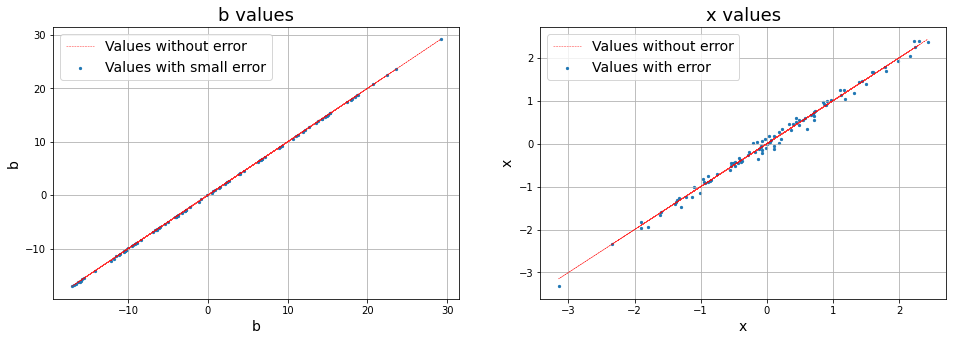
\includegraphics[width=\textwidth]{images/chapter2/ill_condition_demo.png}
	\caption{The influence of the condition number on the solution accuracy}
	\label{fig:ill_condition_demo}
\end{figure}